\chapter[Estado del arte]{\label{identificadorReferenciaCruzada}
Estado del arte}

\section{Los métodos de perspectiva computacional:}

Los principales métodos usados en este campo son algoritmos evolutivos, aprendizaje reforzado, aprendizaje supervisado, aprendizaje no supervisado y búsquedas y planificación en árboles.\\

El aprendizaje supervisado se basa en un modelo de estancias en conjuntos de datos con el objetivo de evaluar las clases, los algoritmos más usados son ID3 o aprendizaje con árboles, redes neuronales y máquinas de soporte vectorial.\\
	
En aprendizaje no supervisado se refiere a búsquedas de patrones, es decir en bases de datos que no tienen valores que nos aporten información directa, los algoritmos más utilizados son el K-medias y auto-organización de mapas.\\

Los algoritmos evolutivos van dirigidos a la optimización estocástica de la generación de la base del juego, los más utilizados son colonias de hormigas y algoritmos genéticos.\\

En la siguiente tabla se muestran las diferentes relaciones entre las investigaciones nombradas anteriormente y los algoritmos usados en esa investigación.\\


\begin{figure}[htb]
  \centering
    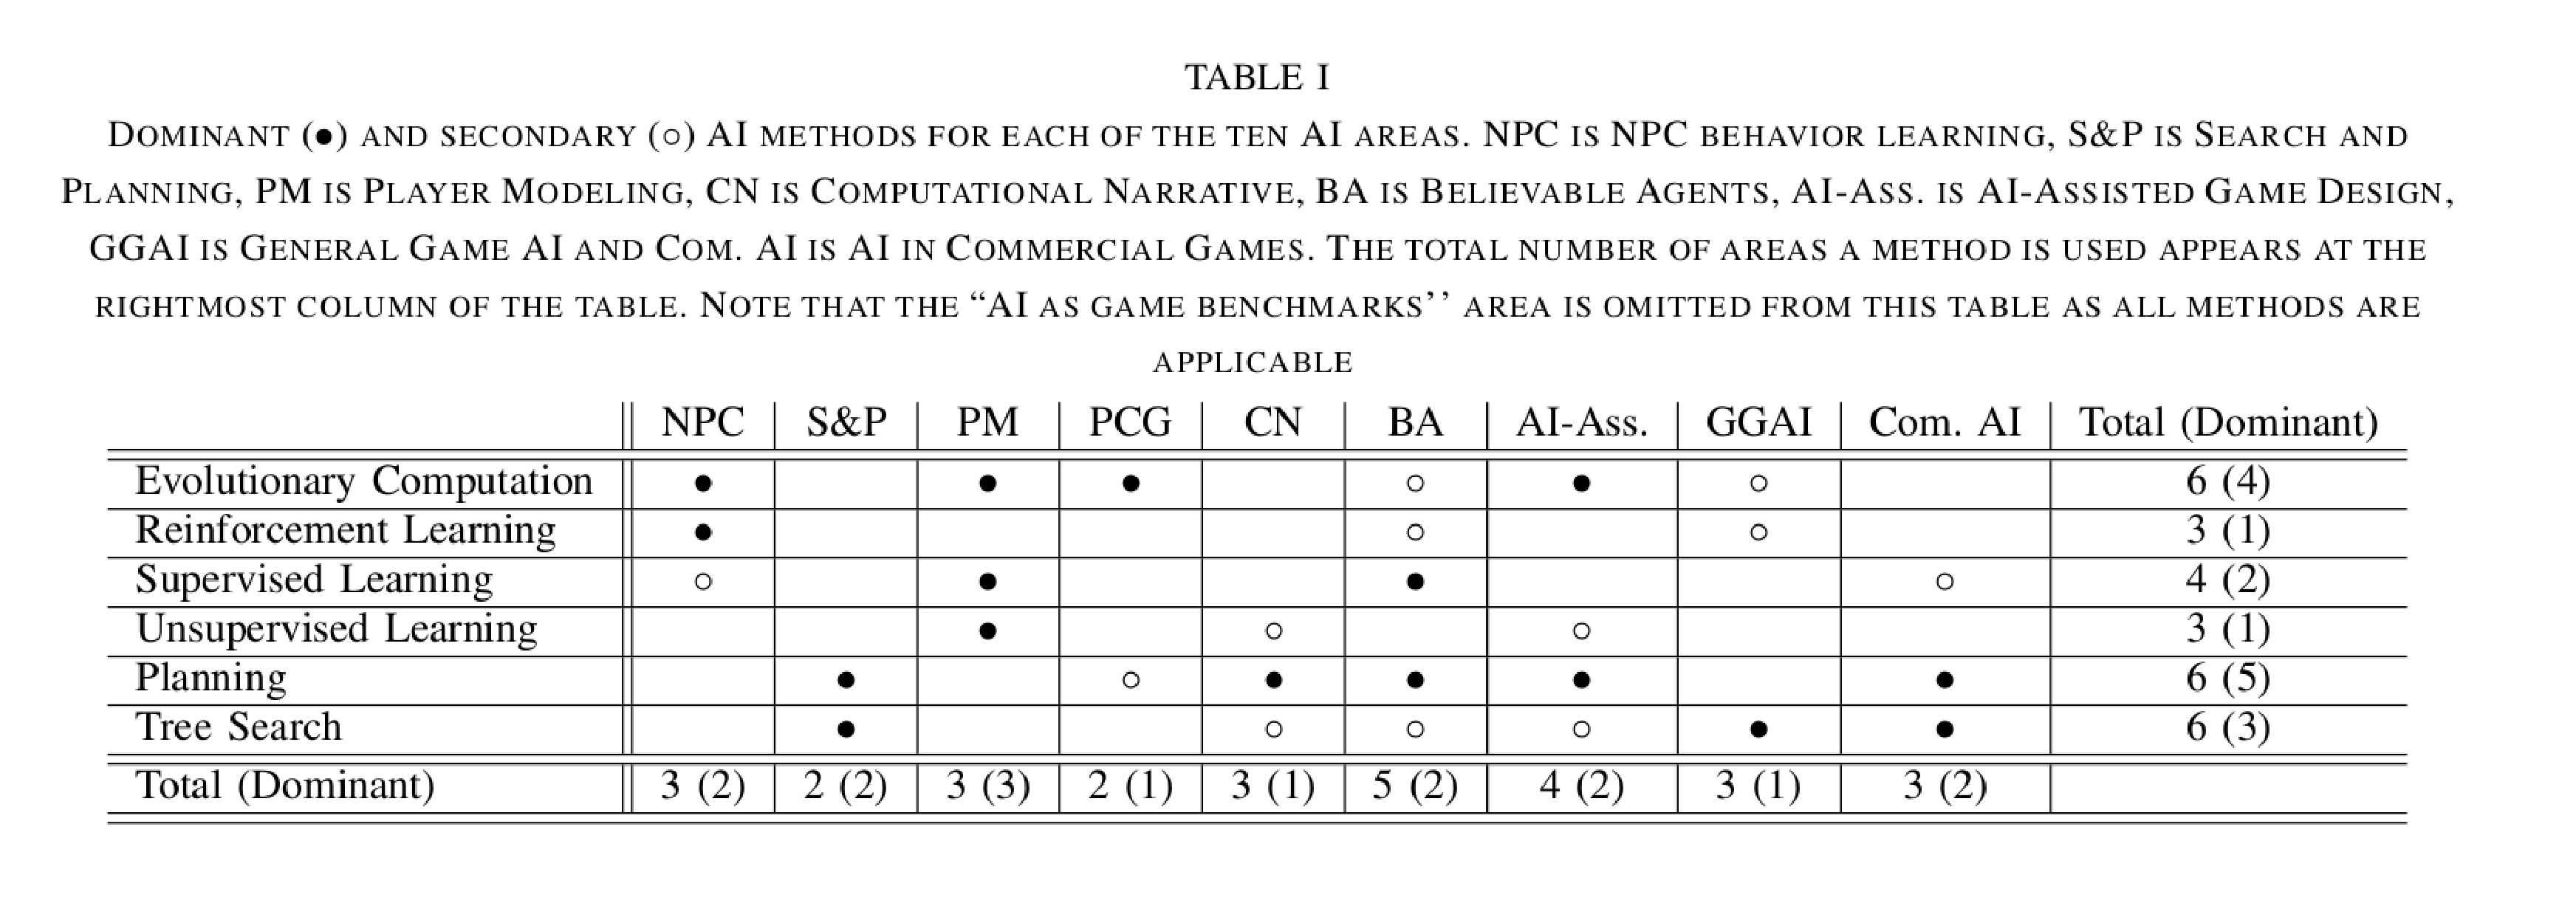
\includegraphics[width=15cm]{./eps/tabla1.eps}
    \vspace{2cm}
  \caption{Tabla1}
  \label{fig:ejemplo}
\end{figure}

\section*{Perspectiva del jugador:}

La perspectiva del jugador se divide en tres dimensiones principales.\\
	
La primera dimensión se basa en ''¿qué puede hacer el jugador con el juego?`` y podemos dividir a su vez, esta dimensión en tres clases, El modelo, generar o evaluar, usuario.

\begin{itemize}

	\item El modelo: Se puede generar gracias a las redes neuronales o a los algoritmos 	genéticos un modelo de juego.\\
		
	\item Generar o evaluar: Se basa en que hay que generar o evaluar en el juego, se pueden 	usar algoritmos para mejorar el juego mientras el jugador esta en interacción con este.\\

	\item Usuario: En esta dimensión se estudia la generación de personajes y el diseño de 	estos.\\  
	
\end{itemize}

\section{Interacción entre las investigaciones:}

Hay varios tipos de influencias, las influencias fuertes y las influencias débiles, por otra parte hay algunas influencias que son bidireccionales, mientras otras son unidireccionales.\\

Uno de los principales nodos de influencia es el aprendizaje del comportamiento del NPC, este comportamiento es aprendido por la IA general del juego y por la interacción del jugador con el juego, por otra parte gracias a ese aprendizaje del comportamiento se genera contenido del juego y modelado de los personajes ya sean NPC o que se modifique el propio personaje que usa el jugador.\\

Por otra parte la planificación y búsquedas también ayudan a la generación de agentes e historias, además de contenido para el juego.\\

En la tabla \ref{fig:ejemplo} aparece la interacción entre las distintas investigaciones:\\

\begin{figure}[htb]
  \centering
    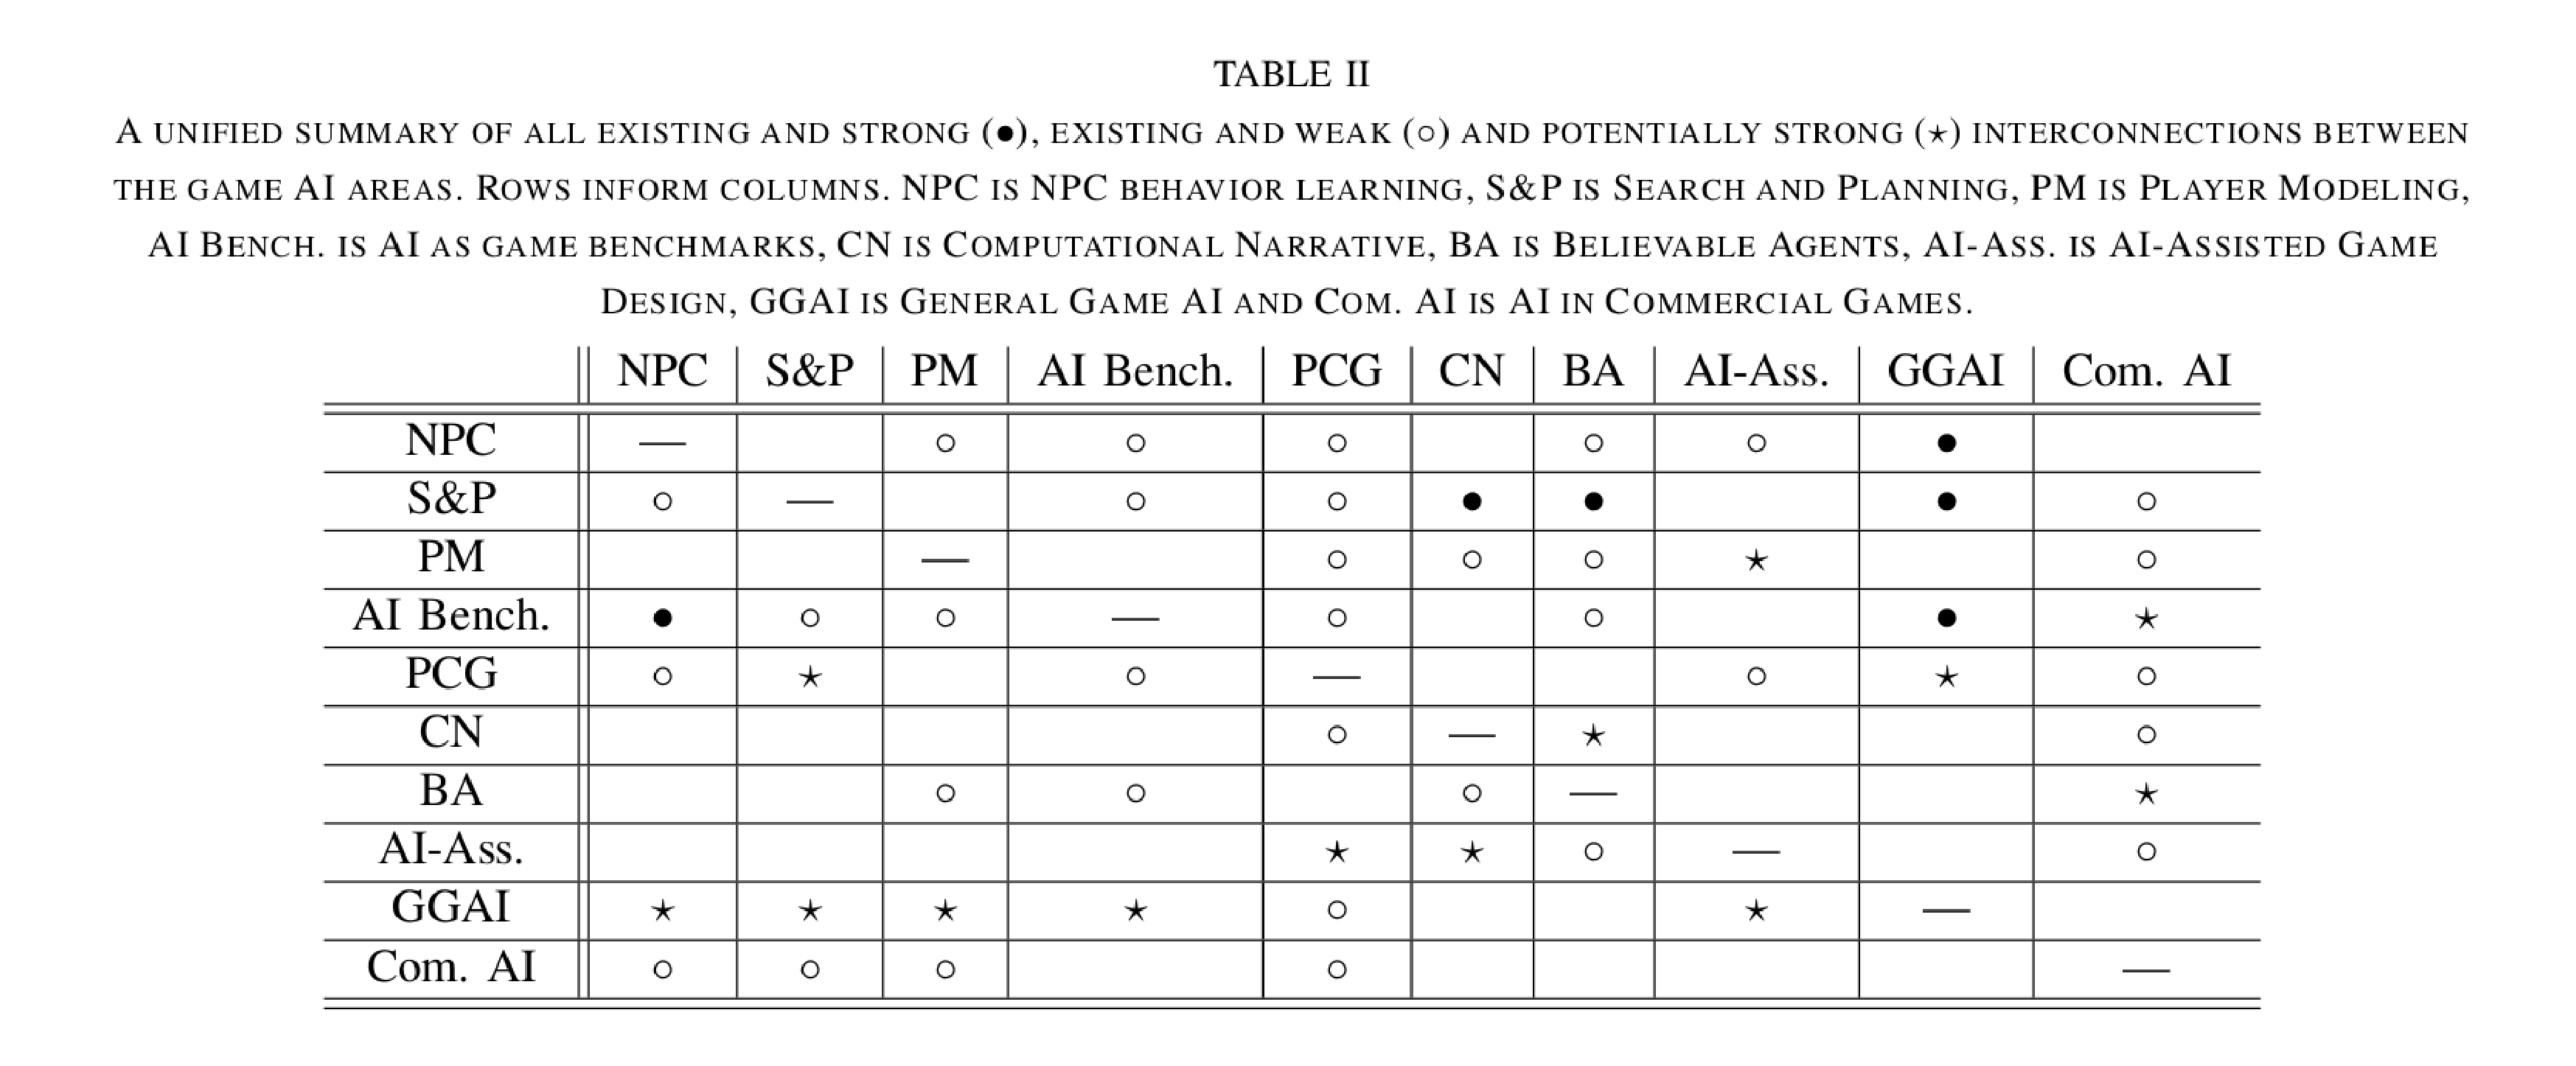
\includegraphics[width=15cm]{./eps/tabla2.eps}
    \vspace{2cm}
  \caption{Tabla2}
  \label{fig:ejemplo}
\end{figure}

\section{Elección:}

Lo que me gustaría hacer de proyecto, es la “AI-ASSISTED GAME DESIGN” para el diseño del juego y principalmente basado en el diseño de ciudades o de mundos, según el juego, es decir como he mostrado anteriormente algoritmos evolutivos para la generación de ciudades o mundos en videojuegos.\\